% Apresentação do HySAIL-R (Online Codes -> Raptor R10 no HySAIL).
% Compilar com scripts/build_presentation.sh (pdflatex, duas passagens).
% Duração prevista: 20 a 30 minutos.
\documentclass[aspectratio=169,10pt]{beamer}

% ---------------------------------------------------------------- Idioma e fontes
\usepackage[T1]{fontenc}
\usepackage[utf8]{inputenc}
% Algumas instalações do TeX Live não trazem o brazil.ldf; nesse caso o babel
% carrega o idioma a partir do arquivo .ini, que acompanha o próprio pacote.
\IfFileExists{brazil.ldf}
	{\usepackage[brazilian]{babel}}
	{\usepackage{babel}\babelprovide[import=pt-BR, main]{brazilian}}
\usepackage[sfdefault]{FiraSans}
\usepackage{amsmath, amssymb}

% ---------------------------------------------------------------- Tema
\usetheme[progressbar=frametitle, numbering=fraction, sectionpage=progressbar, block=fill]{metropolis}

\usepackage{graphicx}
\usepackage{booktabs}
\usepackage{adjustbox}
\usepackage{tikz}

% Diagramas e gráficos reaproveitados da tese e do artigo: uma única fonte.
\graphicspath{{../thesis/img/}{../article/figures/}}
% Estilo comum dos diagramas TikZ da tese.
\usetikzlibrary{arrows.meta,positioning,fit,calc,backgrounds,shapes.geometric,shapes.multipart,decorations.pathreplacing}

% Paleta monocromática: variações de azul, as mesmas dos gráficos de resultados.
% As séries diferem pela luminosidade, e não pelo matiz.
\definecolor{serieA}{HTML}{1F5AA8}
\definecolor{serieB}{HTML}{0B2D63}
\definecolor{serieC}{HTML}{4A8AD4}
\definecolor{serieD}{HTML}{5B7493}
\definecolor{serieE}{HTML}{8FB4E3}
\definecolor{tinta}{HTML}{0B0B0B}
\definecolor{tintaSec}{HTML}{52514E}
\definecolor{fundo}{HTML}{F4F3F0}

\tikzset{
	>={Stealth[length=2.2mm]},
	every node/.style={font=\small},
	caixa/.style={draw=#1!80!black, fill=#1!12, rounded corners=2pt, align=center,
		minimum height=8mm, inner sep=4pt, text=tinta},
	caixa/.default=serieA,
	simbolo/.style={draw=#1!80!black, fill=#1!15, circle, minimum size=8mm,
		inner sep=0pt, text=tinta},
	simbolo/.default=serieA,
	restricao/.style={draw=#1!80!black, fill=#1!25, rectangle, minimum size=6mm,
		inner sep=1pt, text=tinta},
	restricao/.default=serieB,
	seta/.style={->, thick, draw=tintaSec},
	aresta/.style={thick, draw=tintaSec},
	rotulo/.style={font=\footnotesize, text=tintaSec, align=center},
	grupo/.style={draw=tintaSec, dashed, rounded corners=4pt, inner sep=6pt},
	servidor/.style={cylinder, shape border rotate=90, aspect=0.25, draw=serieC!80!black,
		fill=serieC!15, minimum width=13mm, minimum height=11mm, align=center, text=tinta},
}


% Paleta azul das figuras (estilo.tex) aplicada ao tema.
% Fundo branco, igual ao dos gráficos importados.
\setbeamercolor{background canvas}{bg=white}
\setbeamercolor{normal text}{fg=tinta, bg=white}
\setbeamercolor{palette primary}{fg=white, bg=serieB}
\setbeamercolor{frametitle}{bg=serieB, fg=white}
\setbeamercolor{progress bar}{fg=serieC, bg=serieE!40}
\setbeamercolor{alerted text}{fg=serieA}
\setbeamercolor{title separator}{fg=serieC}
\setbeamercolor{block title}{bg=serieE!35, fg=tinta}
\setbeamercolor{block body}{bg=serieE!12}
\setbeamercolor{standout}{bg=serieB, fg=white}
\setbeamertemplate{itemize items}{\color{serieA}\textbullet}
\setbeamertemplate{itemize subitem}{\color{serieC}\textendash}

% Seções com subtítulo: \secao{Título}{Subtítulo}. O subtítulo aparece na
% página de abertura da seção, abaixo da barra de progresso.
% O beamer leva o título longo ao roteiro, que mostra assim também o subtítulo;
% a página de abertura usa o título e o subtítulo guardados separadamente.
\newcommand{\titulosecao}{}
\newcommand{\subtitulosecao}{}
\newcommand{\secao}[2]{%
	\renewcommand{\titulosecao}{#1}\renewcommand{\subtitulosecao}{#2}%
	\section[#1]{\texorpdfstring{#1\protect\hspace{0.8em}{\protect\small\protect\color{tintaSec}#2}}{#1}}}
\setbeamertemplate{section page}{%
	\centering
	\begin{minipage}{24em}
		\raggedright
		\usebeamercolor[fg]{section title}\usebeamerfont{section title}%
		\titulosecao\\[-1ex]
		\usebeamertemplate*{progress bar in section page}\par\vspace{0.6em}
		{\usebeamerfont{subtitle}\color{tintaSec}\subtitulosecao\par}
	\end{minipage}
	\par\vspace{\baselineskip}%
}

% Figura TikZ ajustada à área útil do slide.
\newcommand{\figura}[2][0.72]{%
	\begin{adjustbox}{max width=\textwidth, max totalheight=#1\textheight, center}\input{#2}\end{adjustbox}}
% Coluna de tópicos curtos com espaçamento uniforme.
\newenvironment{topicos}{\begin{itemize}\setlength{\itemsep}{0.7em}}{\end{itemize}}

% ---------------------------------------------------------------- Capa
\title{HySAIL-R}
\subtitle{Substituição de Online Code por Raptor R10}
\author{Ualiton V. Silva \and Dino Macedo Amaral \and João J. C. Gondim}
\institute{Departamento de Ciência da Computação, Universidade de Brasília}
\date{27 de Novembro de 2026}

\begin{document}

\maketitle

\begin{frame}{Roteiro}
	\setbeamertemplate{section in toc}[sections numbered]
	\tableofcontents
\end{frame}

% ================================================================= Motivação
\secao{Motivação}{Dados sob custódia de terceiros}

\begin{frame}{Por que provar que os dados ainda estão lá?}
	\begin{columns}[T, onlytextwidth]
		\column{0.6\textwidth}
		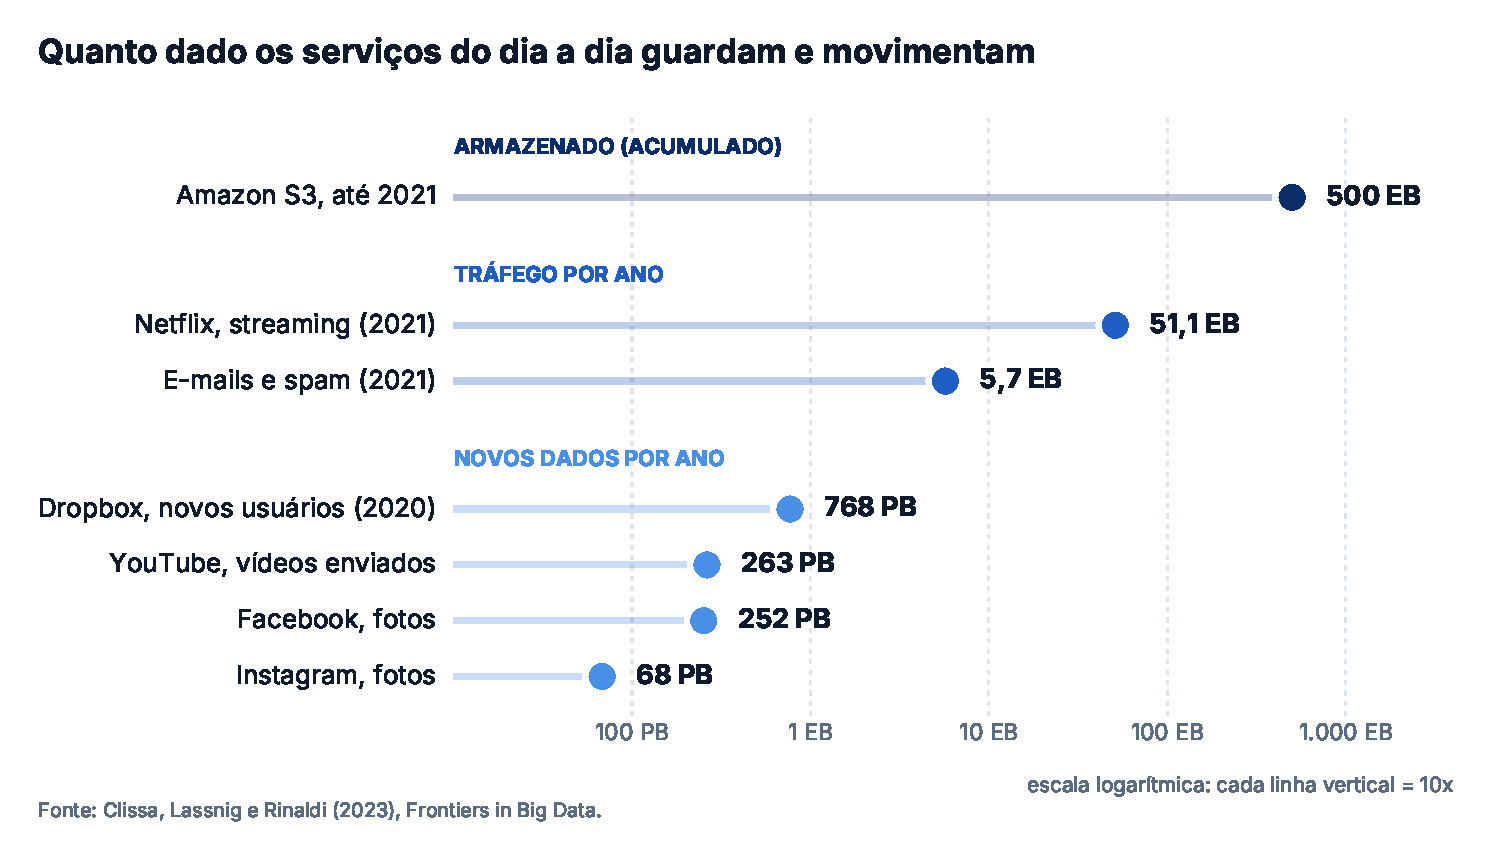
\includegraphics[width=\linewidth]{commercial_data_volumes.pdf}
		\column{0.36\textwidth}
		\begin{itemize}\setlength{\itemsep}{0.4em}
			\item Serviços em nuvem armazenam e transferem dados na ordem de \alert{exabytes}.
			\item Dados podem ser corrompidos ou perdidos \alert{sem aviso}.
			\item Baixar tudo para conferir é inviável.
			\item \textbf{Prova de recuperabilidade (PoR):} verifica por \alert{amostragem} que o arquivo ainda é recuperável.
		\end{itemize}
	\end{columns}
\end{frame}

% ================================================================= HySAIL
\secao{HySAIL}{Provas de recuperabilidade em múltiplas nuvens}

\begin{frame}{HySAIL: usuário, provedores e cinco fases}
	\figura[0.68]{../thesis/img/tikz/hysail_protocolo}
	\vfill
	\centering
	O usuário guarda só \alert{metadados}, e os provedores guardam os blocos.
\end{frame}

\begin{frame}{O MAC homomórfico ao XOR}
	\figura[0.5]{../thesis/img/tikz/mac_homomorfico}
	\vfill
	\begin{topicos}
		\item MAC de um bloco: $h_{i,j} = m_i(x) \bmod P_j(x)$, com $P_j$ primitivo de grau 127.
		\item Todo bloco codificado é um XOR de blocos de mensagem $\Rightarrow$ seu MAC é o XOR dos MACs.
		\item Auditoria: o provedor responde $\left(\bigoplus c_\eta\right) \bmod P_j$, e o usuário confere.
	\end{topicos}
\end{frame}

% ================================================================= Códigos
\secao{Códigos fountain}{Do LT Codes ao Raptor R10}

\begin{frame}{Códigos \emph{fountain}: a ideia comum}
	\begin{columns}[c, onlytextwidth]
		\column{0.55\textwidth}
		\begin{topicos}
			\item $K$ símbolos de origem geram uma quantidade \alert{ilimitada} de símbolos codificados.
			\item O receptor não escolhe quais símbolos recebe: basta receber \alert{pouco mais de $K$}.
			\item \textbf{\emph{Overhead} de recepção:} quantos símbolos além de $K$ são necessários para decodificar.
			\item Todas as operações são XOR em $GF(2)$: cada símbolo codificado é a soma de símbolos de origem.
		\end{topicos}
		\column{0.4\textwidth}
		\begin{block}{Por que isso importa ao HySAIL}
			\small
			Se $c = d_a \oplus d_b$, então
			\[ \mathrm{MAC}(c) = \mathrm{MAC}(d_a) \oplus \mathrm{MAC}(d_b). \]
			O usuário verifica \alert{qualquer} símbolo codificado guardando só os MACs dos símbolos de origem.
		\end{block}
	\end{columns}
\end{frame}

\begin{frame}{LT Codes: codificação}
	\begin{columns}[T, onlytextwidth]
		\column{0.46\textwidth}
		Para gerar o símbolo codificado $c_i$:
		\begin{enumerate}\setlength{\itemsep}{0.5em}
			\item Sorteia um grau $\delta_i$ da distribuição \alert{sóliton robusta}.
			\item Escolhe $\delta_i$ símbolos de origem distintos, de índices $S_i$.
			\item Calcula $c_i = \bigoplus_{j \in S_i} d_j$.
			\item Envia a semente do gerador, para que o receptor reproduza $S_i$.
		\end{enumerate}
		\vspace{0.5em}
		Graus baixos iniciam a decodificação, e graus altos garantem que todo símbolo seja coberto.
		\column{0.5\textwidth}
		\begin{block}{Exemplo com $K = 3$}
			\small
			$d_1 = 1010,\ d_2 = 0110,\ d_3 = 1101$
			\par\vspace{0.6em}
			\renewcommand{\arraystretch}{1.25}
			\setlength{\tabcolsep}{3pt}
			\begin{tabular}{@{}ll@{}}
				$S_1 = \{2\}$ & $c_1 = d_2 = 0110$ \\
				$S_2 = \{1, 2\}$ & $c_2 = d_1 \oplus d_2 = 1100$ \\
				$S_3 = \{1, 2, 3\}$ & $c_3 = d_1 \oplus d_2 \oplus d_3 = 0001$ \\
			\end{tabular}
		\end{block}
	\end{columns}
\end{frame}

\begin{frame}{LT Codes: decodificação por \emph{peeling}}
	\figura[0.42]{../thesis/img/tikz/lt_grafo}
	\vfill
	\begin{topicos}
		\item Um símbolo de grau 1 revela um símbolo de origem, removido por XOR dos vizinhos.
		\item Cada remoção reduz graus e pode criar novos símbolos de grau 1. Sem eles, o processo para.
		\item Simples e rápido, mas exige graus até $K$ e muitos símbolos extras: \alert{17\% a 56\%} de $K$.
	\end{topicos}
\end{frame}

\begin{frame}{Online Codes: código externo e código interno}
	\begin{columns}[T, onlytextwidth]
		\column{0.5\textwidth}
		\textbf{Código externo} (\emph{outer code})
		\begin{itemize}\setlength{\itemsep}{0.4em}
			\item Cria $m$ símbolos auxiliares, cada um o XOR de símbolos de origem:
			\[ a_l = \bigoplus_{j \in A_l} d_j \]
			\item Cada símbolo de origem $d_j$ é sorteado para \alert{3 símbolos auxiliares} ($q = 3$, o fator de repetição).
			\item Forma a mensagem composta $\mathbf{v} = (d_1, \ldots, d_K, a_1, \ldots, a_m)$.
		\end{itemize}
		\column{0.46\textwidth}
		\textbf{Código interno} (\emph{inner code})
		\begin{itemize}\setlength{\itemsep}{0.4em}
			\item Gera blocos de verificação como o LT, mas sobre $\mathbf{v}$.
			\item O grau máximo é \alert{constante}, independente de $K$.
			\item Codificação e decodificação em tempo \alert{linear}.
		\end{itemize}
	\end{columns}
	\vfill
	\centering
	O grau limitado só recupera \emph{quase} toda a mensagem, e o código externo completa o restante.
\end{frame}

\begin{frame}{Online Codes: decodificação em duas etapas}
	\figura[0.48]{../thesis/img/tikz/online_codes}
	\vfill
	\begin{topicos}
		\item \textbf{1.} \emph{Peeling} sobre os blocos de verificação recupera quase todo $\mathbf{v}$.
		\item \textbf{2.} As relações $a_l = \bigoplus d_j$ recuperam os símbolos de origem restantes.
		\item Recupera com $\approx (1 + 3\varepsilon)K$ blocos: o excedente $3\varepsilon K$ \alert{cresce com $K$}.
	\end{topicos}
\end{frame}

\begin{frame}{Online Codes: limitações para o HySAIL}
	\begin{topicos}
		\item \textbf{Não sistemáticos:} os dados originais não são armazenados diretamente, então ler o arquivo exige decodificar.
		\item \textbf{Excedente alto para $K$ pequeno:} \alert{65\%} com $K = 10$ e \alert{34\%} com $K = 100$.
		\item \textbf{Quantidade de blocos aleatória:} com $K = 100$, o codificador grava blocos até o \emph{chunk} decodificar, \alert{143} em vez de 125.
		\item \textbf{Consequência no HySAIL original:} o arquivo inteiro é codificado de uma vez, para diluir o excedente, e o reparo deixa de ser local a uma parte do arquivo.
	\end{topicos}
\end{frame}

\begin{frame}{Raptor R10: visão geral}
	\figura[0.42]{../thesis/img/tikz/raptor_r10}
	\vfill
	\begin{itemize}\setlength{\itemsep}{0.4em}
		\item Padronizado na \alert{RFC 5053}, para $4 \le K \le 8.192$ símbolos de origem.
		\item Pré-codificação: $K$ símbolos de origem $\rightarrow$ $L = K + S + H$ símbolos intermediários.
		\item Codificação LT sobre os intermediários, em que o conjunto de cada bloco depende só de $K$ e do \alert{ESI} $\eta$.
		\item Custo: \alert{quase linear} em $K$ pela norma, e quadrático no pior caso, detalhado adiante.
	\end{itemize}
\end{frame}

\begin{frame}{Raptor R10: pré-codificação com símbolos LDPC}
	\begin{columns}[T, onlytextwidth]
		\column{0.56\textwidth}
		\begin{itemize}\setlength{\itemsep}{0.35em}
			\item \textbf{O que são:} $S$ símbolos de \alert{paridade}, $C_K, \ldots, C_{K+S-1}$, criados pela pré-codificação.
			\item \textbf{Quantos:} $X$ é o menor inteiro com $X(X-1) \ge 2K$, e $S$ é o menor primo $\ge \lceil 0{,}01K \rceil + X$.
			\item \textbf{Quem entra:} cada $C_i$, com $i < K$, entra em \alert{3} símbolos LDPC, nas posições $b$, $b + a$ e $b + 2a \pmod S$, com
			\[ b = i \bmod S, \quad a = 1 + (\lfloor i/S \rfloor \bmod (S - 1)). \]
			\item Cada símbolo LDPC é o XOR dos $C_i$ que caem na sua posição.
		\end{itemize}
		\column{0.41\textwidth}
		\begin{block}{Exemplo com $K = 10$}
			\small
			$X = 5$, pois $5 \cdot 4 \ge 20$. $S = 7$, o primo $\ge 6$.
			\par\vspace{0.4em}
			\centering
			\renewcommand{\arraystretch}{1.1}
			\begin{tabular}{rrrl}
				$i$ & $a$ & $b$ & posições \\
				\midrule
				0 & 1 & 0 & \alert{0}, 1, 2 \\
				5 & 1 & 5 & 5, 6, \alert{0} \\
				6 & 1 & 6 & 6, \alert{0}, 1 \\
				7 & 2 & 0 & \alert{0}, 2, 4 \\
				8 & 2 & 1 & 1, 3, 5 \\
			\end{tabular}
			\par\vspace{0.5em}
			\raggedright
			Posição 0: $C_{10} = C_0 \oplus C_5 \oplus C_6 \oplus C_7$.
		\end{block}
	\end{columns}
\end{frame}

\begin{frame}{Raptor R10: pré-codificação com símbolos Half}
	\begin{columns}[T, onlytextwidth]
		\column{0.53\textwidth}
		\begin{itemize}\setlength{\itemsep}{0.45em}
			\item \textbf{O que são:} $H$ símbolos de paridade \alert{densos}, $C_{K+S}, \ldots, C_{L-1}$, com $L = K + S + H$.
			\item \textbf{Quantos:} $H$ é o menor inteiro com $\binom{H}{\lceil H/2 \rceil} \ge K + S$.
			\item \textbf{Quem entra:} cada $C_j$, com $j < K + S$ (origem e LDPC), recebe um código de $H$ bits com exatamente $\lceil H/2 \rceil$ bits 1, tirado da sequência de Gray $g(n) = n \oplus \lfloor n/2 \rfloor$.
			\item Os bits 1 indicam em quais símbolos Half $C_j$ entra, ou seja, em \alert{metade} deles.
		\end{itemize}
		\column{0.43\textwidth}
		\begin{block}{Exemplo com $K = 10$, $S = 7$}
			\small
			$\binom{5}{3} = 10 < 17 \le \binom{6}{3} = 20$, então $H = 6$ e $L = 23$.
			\par\vspace{0.4em}
			\centering
			\renewcommand{\arraystretch}{1.1}
			\begin{tabular}{rll}
				$j$ & código & símbolos Half \\
				\midrule
				0 & 000111 & 0, 1, 2 \\
				1 & 001101 & 0, 2, 3 \\
				2 & 001110 & 1, 2, 3 \\
				3 & 001011 & 0, 1, 3 \\
			\end{tabular}
			\par\vspace{0.5em}
			\raggedright
			Com $K = 100$: $S = 17$, $H = 9$, $L = \alert{126}$.
		\end{block}
	\end{columns}
\end{frame}

\begin{frame}{Raptor R10: código sistemático e decodificação}
	\begin{columns}[c, onlytextwidth]
		\column{0.42\textwidth}
		\centering
		$A \cdot C = D$\\[0.6em]
		$A = \begin{bmatrix}
			G_{LDPC} & I_S & 0 \\
			\multicolumn{2}{c}{G_{Half}} & I_H \\
			\multicolumn{3}{c}{G_{LT}}
		\end{bmatrix}$\\[0.6em]
		{\small $D$: $S + H$ zeros seguidos dos $K$ símbolos de origem}
		\column{0.54\textwidth}
		\begin{topicos}
			\item Os intermediários $C$ são escolhidos para que os ESIs $0, \ldots, K-1$ \alert{reproduzam os dados}.
			\item Todo bloco é XOR de símbolos de origem: $c_\eta = \bigoplus_{i \in X_\eta} d_i$, com suporte $X_\eta$.
			\item Decodificação por eliminação gaussiana em $GF(2)$: recupera se os suportes recebidos têm \alert{posto $K$}.
			\item Não é MDS: com $K = 100$, exatamente $K$ blocos falham em 75\% dos casos. Em média bastam \alert{$K + 1{,}8$}, e sempre bastaram $K + 12$.
		\end{topicos}
	\end{columns}
\end{frame}

\begin{frame}{Raptor R10: complexidade}
	\small
	Custo em XORs de símbolos de $T$ bytes, para um \emph{chunk} de $K$ símbolos:
	\par\vspace{0.6em}
	\centering
	\renewcommand{\arraystretch}{1.3}
	\begin{tabular}{@{}lll@{}}
		\toprule
		\textbf{Código} & \textbf{Codificação} & \textbf{Decodificação} \\
		\midrule
		LT Codes & $O(K \log K \cdot T)$ & $O(K \log K \cdot T)$ \\
		Online Codes & $O(K \cdot T)$ & $O(K \cdot T)$ \\
		R10, RFC 5053 (inativação) & $\approx O(K \cdot T)$ na prática & $\approx O(K \cdot T)$ na prática \\
		R10, HySAIL-R (eliminação direta) & $O(\varepsilon K^2 \cdot T)$ & $O(K^2 \cdot T)$ no pior caso \\
		\bottomrule
	\end{tabular}
	\par\vspace{0.8em}
	\raggedright
	\begin{itemize}\setlength{\itemsep}{0.35em}
		\item Resolver $A \cdot C = D$ custa $O(L^3)$ operações de bit, \alert{não depende de $T$} e é feito uma vez por $K$.
		\item No HySAIL-R, cada bloco de reparo é o XOR de $\approx K/2$ símbolos de origem, daí o termo $K^2$.
		\item Com $K = 100$, isso pesa pouco: \alert{2,8 ms} para codificar e \alert{3,5 ms} para decodificar um \emph{chunk}, contra 2,6 e 3,2 ms dos Online Codes.
	\end{itemize}
\end{frame}

\begin{frame}{Raptor R10: exemplo simplificado de recuperação}
	\begin{columns}[T, onlytextwidth]
		\column{0.48\textwidth}
		\textbf{Codificação}
		\par\vspace{0.4em}
		$d_1 = 1010,\ d_2 = 0110,\ d_3 = 1101$\\
		Pré-código: $C_4 = d_1 \oplus d_2 \oplus d_3 = 0001$
		\par\vspace{0.6em}
		\renewcommand{\arraystretch}{1.25}
		\begin{tabular}{@{}lll@{}}
			$c_1 = C_1$ & $= 1010$ & $X_1 = \{1\}$ \\
			$c_2 = C_2 \oplus C_3$ & $= 1011$ & $X_2 = \{2, 3\}$ \\
			$c_3 = C_2 \oplus C_4$ & $= 0111$ & $X_3 = \{1, 3\}$ \\
		\end{tabular}
		\column{0.48\textwidth}
		\textbf{Recuperação}
		\begin{itemize}\setlength{\itemsep}{0.4em}
			\item Suportes como vetores: $100$, $011$, $101$ $\Rightarrow$ \alert{posto 3}.
			\item $d_1 = c_1 = 1010$
			\item $d_3 = c_3 \oplus d_1 = 1101$
			\item $d_2 = c_2 \oplus d_3 = 0110$
		\end{itemize}
	\end{columns}
	\vfill
	\centering
	Mesmo os blocos que passam pelo pré-código continuam sendo \alert{XOR de símbolos de origem}.
\end{frame}

\begin{frame}{Distribuições de grau dos três códigos}
	\begin{columns}[c, onlytextwidth]
		\column{0.55\textwidth}
		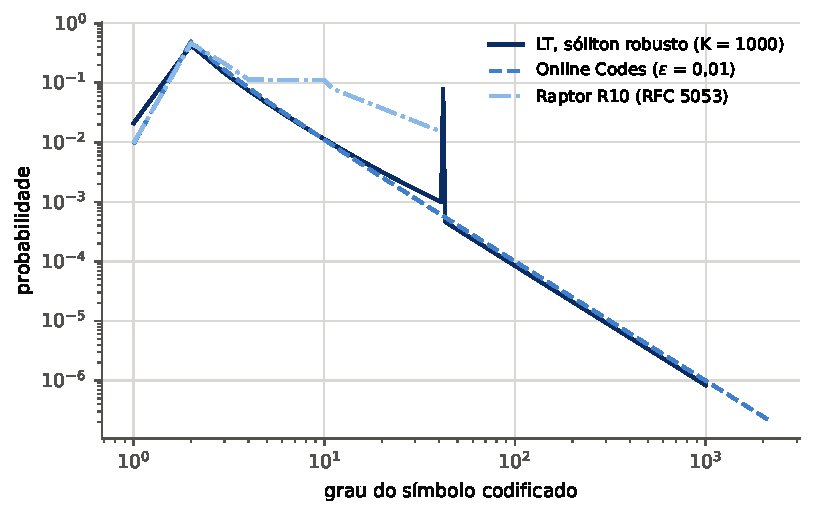
\includegraphics[width=\linewidth]{resultados/degree_distributions.pdf}
		\column{0.42\textwidth}
		\begin{topicos}
			\item \textbf{LT:} graus até $K$, com grau médio \alert{10,3}.
			\item \textbf{Online:} grau máximo constante, mas alto (2.115), com média \alert{8,2}.
			\item \textbf{R10:} só os graus 1, 2, 3, 4, 10, 11 e 40, com média \alert{4,6}.
			\item O pré-código cobre o que a etapa LT deixa de alcançar.
		\end{topicos}
	\end{columns}
\end{frame}

% ================================================================= Proposta
\secao{HySAIL-R}{O que muda em relação ao HySAIL original}

\begin{frame}{Mudanças em relação ao HySAIL}
	\begin{columns}[T, onlytextwidth]
		\column{0.56\textwidth}
		\begin{block}{Mudou}
			\begin{itemize}\setlength{\itemsep}{0.35em}
				\item Online Codes $\rightarrow$ \alert{Raptor R10} (RFC 5053).
				\item Arquivo inteiro $\rightarrow$ \alert{\emph{chunks}} de $K = 100$ símbolos.
				\item Composição $\langle i, x_i\rangle$ armazenada $\rightarrow$ derivada de $(K, \eta)$.
				\item Recuperabilidade avaliada pelo \alert{posto $K$}.
				\item Reparo gera um \alert{ESI inédito}, sem decodificar.
			\end{itemize}
		\end{block}
		\column{0.4\textwidth}
		\begin{block}{Mantido}
			\begin{itemize}\setlength{\itemsep}{0.35em}
				\item MAC homomórfico ao XOR.
				\item Auditoria nos modelos limitado e ilimitado.
				\item Redistribuição local.
				\item Múltiplos provedores.
				\item Desafios $P_j$ primitivos de grau 127, agora verificados pelo teste de Rabin.
			\end{itemize}
		\end{block}
	\end{columns}
\end{frame}

\begin{frame}{MAC derivado e modelos de auditoria}
	\begin{columns}[T, onlytextwidth]
		\column{0.42\textwidth}
		O MAC de \alert{qualquer} bloco R10, inclusive os gerados no reparo, vem dos MACs de origem:
		\[ h_{\eta,j}(x) = \bigoplus_{i \in X_\eta} h_{i,j}(x) \]
		O suporte $X_\eta$ é recalculado a partir de $(K, \eta)$, e nada além dos MACs de origem é guardado.
		\column{0.54\textwidth}
		\footnotesize
		\renewcommand{\arraystretch}{1.3}
		\setlength{\tabcolsep}{3pt}
		\begin{tabular*}{\linewidth}{@{\extracolsep{\fill}}lll@{}}
			\toprule
			& \textbf{Limitado} & \textbf{Ilimitado} \\
			\midrule
			Polinômios & $l = 40$, uso único & 1, secreto \\
			MACs do usuário & $n \cdot l$ & $n$ \\
			Desafio & $P_j$ e blocos & só os blocos \\
			Resposta & $\left(\bigoplus c_\eta\right) \bmod P_j$ & $\bigoplus c_\eta$ \\
			Tamanho da resposta & 16 bytes & $\approx$ 1 bloco \\
			Quem reduz mod $P$ & provedor & usuário \\
			Auditorias & 40 & ilimitadas \\
			\bottomrule
		\end{tabular*}
	\end{columns}
\end{frame}

\begin{frame}{\emph{Chunks}, $K$ e paralelização}
	\figura[0.86]{figuras/chunks_paralelizacao}
	\vfill
	\centering
	\small Com $\varepsilon = 0{,}25$, $r = \lceil \varepsilon K \rceil = 25$, e cada \emph{chunk} gera $K + r = 125$ blocos.
\end{frame}

\begin{frame}{Redistribuição sem decodificar o \emph{chunk}}
	\figura[0.6]{figuras/redistribuicao}
	\vfill
	\centering
	Cada reparo transfere $\approx$ \alert{49 blocos (320 KB)}, qualquer que seja o tamanho do arquivo.
\end{frame}

% ================================================================= Resultados
\secao{Métricas}{Medidas em cada fase do HySAIL-R}

\begin{frame}{Recuperação: \emph{overhead} de recepção}
	\begin{columns}[c, onlytextwidth]
		\column{0.55\textwidth}
		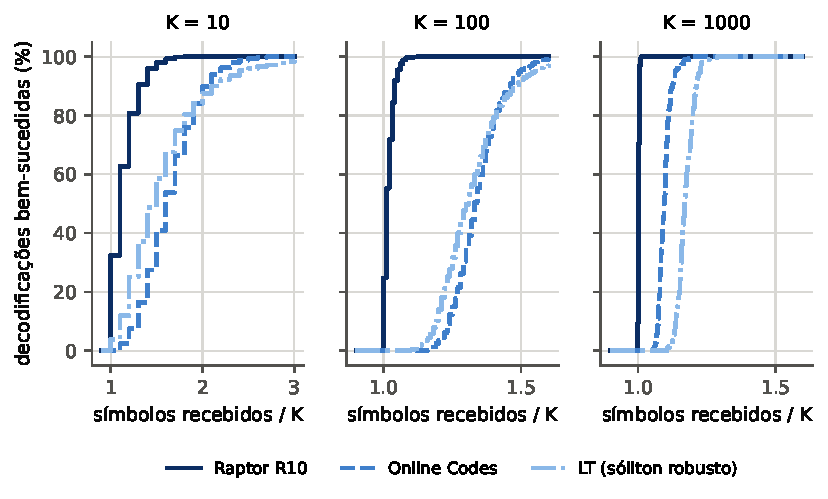
\includegraphics[width=\linewidth]{resultados/reception_overhead.pdf}
		\column{0.42\textwidth}
		\footnotesize
		Símbolos extras, em \% de $K$ (média)
		\par\vspace{0.4em}
		\begin{tabular*}{\linewidth}{@{\extracolsep{\fill}}lrrr@{}}
			\toprule
			$K$ & \textbf{R10} & \textbf{Online} & \textbf{LT} \\
			\midrule
			10 & \alert{14\%} & 65\% & 56\% \\
			100 & \alert{1,8\%} & 34\% & 32\% \\
			1.000 & \alert{0,27\%} & 9,7\% & 17\% \\
			\bottomrule
		\end{tabular*}
		\par\vspace{0.8em}
		\small
		No R10, o excedente é quase \alert{constante}: 1,4 a 2,7 símbolos. Por isso $K = 100$ já basta.
	\end{columns}
\end{frame}

\begin{frame}{Redundância: tolerância a perdas e tamanho do \emph{chunk}}
	\begin{columns}[c, onlytextwidth]
		\column{0.5\textwidth}
		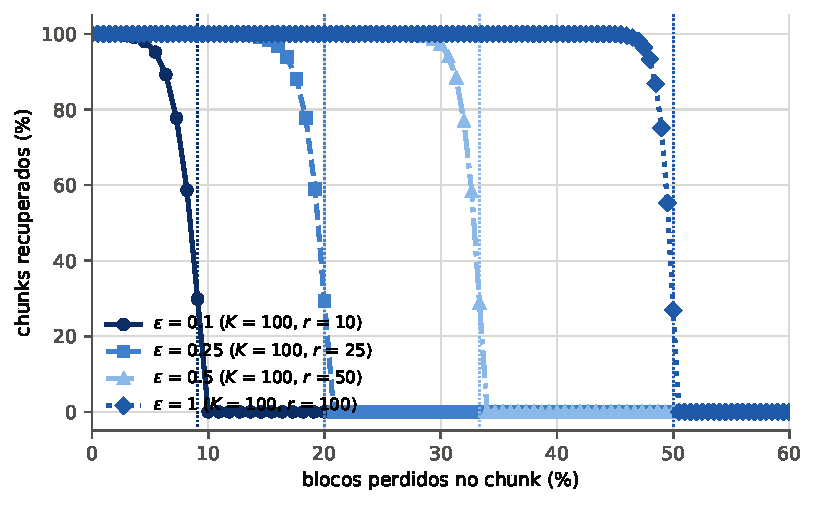
\includegraphics[width=\linewidth]{figuras/resultados/loss_tolerance.pdf}
		\column{0.47\textwidth}
		\footnotesize
		\begin{tabular*}{\linewidth}{@{\extracolsep{\fill}}rrrr@{}}
			\toprule
			$K$ & $\varepsilon$ & \textbf{Perda tolerada} & \textbf{Reparo} \\
			\midrule
			10 & 0,25 & 0\% & 33 KB \\
			10 & 0,5 & 6,7\% & 33 KB \\
			100 & 0,25 & \alert{14,4\%} & \alert{325 KB} \\
			100 & 0,5 & 28,7\% & 325 KB \\
			250 & 0,25 & 17,9\% & 813 KB \\
			1.000 & 0,25 & 19,5\% & 3,3 MB \\
			\bottomrule
		\end{tabular*}
		\par\vspace{0.6em}
		\small
		$K = 100$ fica perto do limite MDS de 20\% com um reparo ainda barato.
	\end{columns}
\end{frame}

\begin{frame}{Codificação: onde o tempo é gasto}
	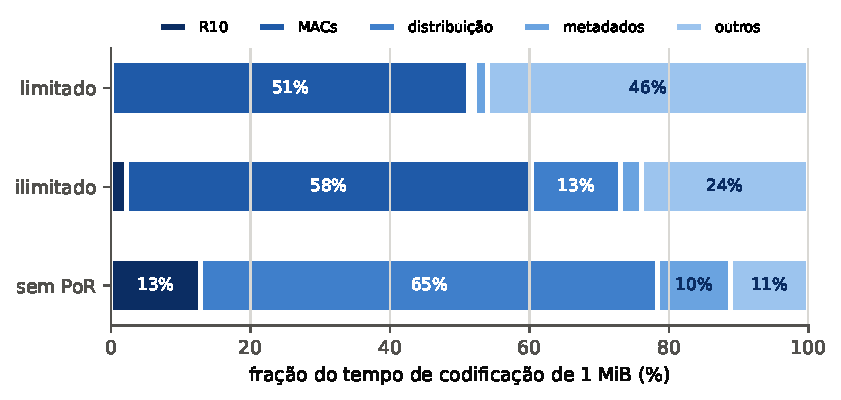
\includegraphics[width=\linewidth, height=0.36\textheight, keepaspectratio]{resultados/encode_stages.pdf}
	\vfill
	\begin{columns}[T, onlytextwidth]
		\column{0.48\textwidth}
		\begin{itemize}\setlength{\itemsep}{0.4em}
			\item O R10 custa só \alert{13\%} da codificação sem PoR, enquanto gravar nos provedores custa cerca de 2/3.
			\item Um MAC de 6.500 bytes custa $\approx$ \alert{0,1 ms}.
		\end{itemize}
		\column{0.48\textwidth}
		\begin{itemize}\setlength{\itemsep}{0.4em}
			\item 1 MiB: \alert{4,4 s} no limitado (40 polinômios) e \alert{0,11 s} no ilimitado.
			\item 64 MiB: 1,6 s sem PoR e 7,0 s no ilimitado, crescendo linearmente.
		\end{itemize}
	\end{columns}
\end{frame}

\begin{frame}{Auditoria: probabilidade de detecção}
	\begin{columns}[T, onlytextwidth]
		\column{0.52\textwidth}
		Em cada rodada, o usuário sorteia blocos de um provedor e confere o XOR deles. Basta \alert{um} bloco corrompido na amostra para a resposta não bater.
		\par\vspace{0.6em}
		\begin{itemize}\setlength{\itemsep}{0.3em}
			\item $N$: blocos guardados no provedor.
			\item $c$: blocos corrompidos, e $\beta = c/N$ é a fração corrompida.
			\item $s$: blocos sorteados na auditoria.
		\end{itemize}
		\[ P(\text{detectar}) = 1 - \frac{\binom{N-c}{s}}{\binom{N}{s}} \]
		{\small A fração é a chance de sortear \alert{só blocos íntegros}.}
		\column{0.44\textwidth}
		\begin{block}{Exemplo: arquivo de 4 MiB, $N = 294$}
			\small
			$c = 3$ ($\beta = 1\%$), $s = 50$:
			\[ \frac{244 \cdot 243 \cdot 242}{294 \cdot 293 \cdot 292} \approx 0{,}57 \]
			$\Rightarrow P \approx \alert{43\%}$.
			\par\vspace{0.6em}
			$c = 15$ ($\beta = 5{,}1\%$), $s = 50$: $P \approx \alert{94\%}$.
			\par\vspace{0.6em}
			Quanto menor $\beta$, maior precisa ser $s$.
		\end{block}
	\end{columns}
\end{frame}

\begin{frame}{Auditoria: detecção medida}
	\begin{columns}[c, onlytextwidth]
		\column{0.5\textwidth}
		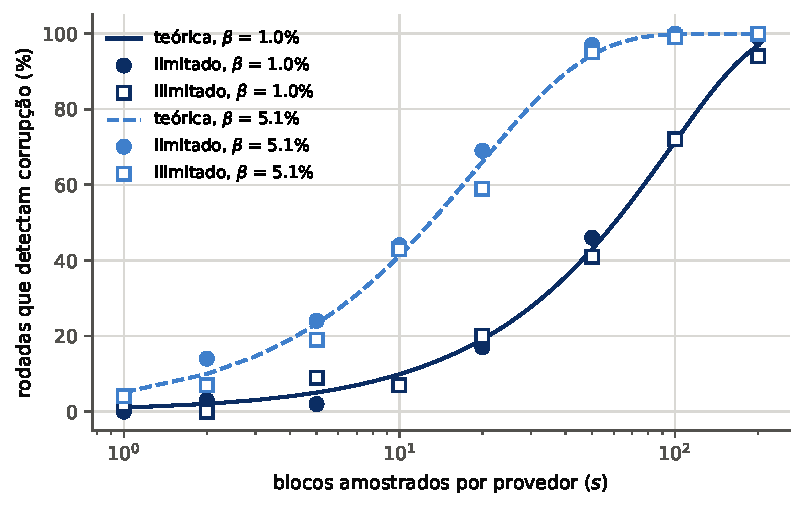
\includegraphics[width=\linewidth]{figuras/resultados/audit_detection.pdf}
		\column{0.47\textwidth}
		\begin{itemize}\setlength{\itemsep}{0.5em}
			\item Curvas: a fórmula $P$. Pontos: 100 rodadas medidas para cada $s$.
			\item $\beta = 5{,}1\%$, $s = 50$: detecta em \alert{97\%} (limitado) e \alert{95\%} (ilimitado), com teoria de 94\%.
			\item $\beta = 1\%$: são precisos $s = 200$ blocos para 94\% a 99\%.
			\item Rodada com $s = 50$ (1 MiB): \alert{10 ms} no ilimitado e 0,15 s no limitado.
			\item Com o \alert{mesmo erro} em todos os blocos, o XOR cancela erros e a detecção cai para 48\%--74\%.
		\end{itemize}
	\end{columns}
\end{frame}

\begin{frame}{Memória do usuário e armazenamento}
	\begin{columns}[c, onlytextwidth]
		\column{0.5\textwidth}
		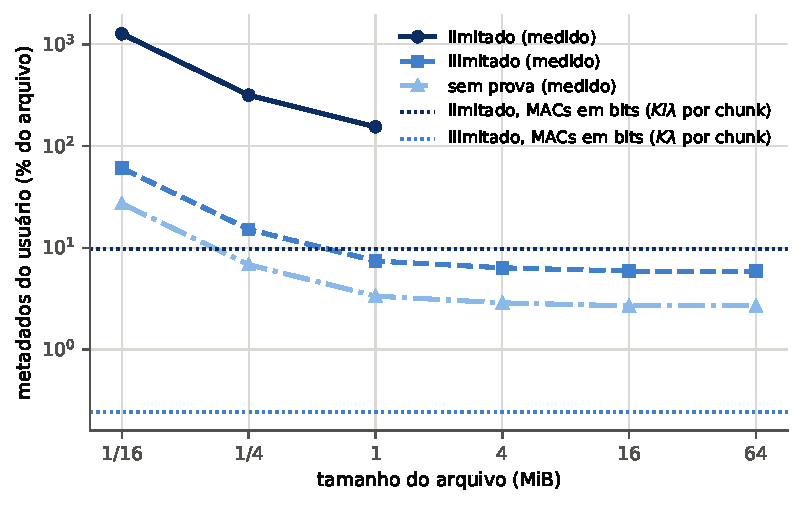
\includegraphics[width=\linewidth]{resultados/metadata_size.pdf}
		\column{0.47\textwidth}
		\footnotesize
		Arquivo de 1 MiB, 2 \emph{chunks}, 250 blocos
		\par\vspace{0.4em}
		\begin{tabular*}{\linewidth}{@{\extracolsep{\fill}}lrr@{}}
			\toprule
			& \textbf{Limitado} & \textbf{Ilimitado} \\
			\midrule
			MACs do usuário & 8.000 & 200 \\
			Metadados / arquivo & 154,5\% & \alert{7,4\%} \\
			Decodificação & 0,20 s & 0,03 s \\
			\bottomrule
		\end{tabular*}
		\par\vspace{0.6em}
		\small
		No ilimitado, os metadados convergem para \alert{5,9\%} do arquivo, e os provedores guardam \alert{1,27$\times$} o arquivo.
	\end{columns}
\end{frame}

\begin{frame}{Redistribuição e limitações medidas}
	\begin{columns}[T, onlytextwidth]
		\column{0.48\textwidth}
		\textbf{Redistribuição}
		\begin{topicos}
			\item Cada bloco reparado transfere $\approx$ \alert{49 blocos (320 KB)}.
			\item O custo depende do \emph{chunk}, não do tamanho do arquivo.
			\item O novo bloco não exige novos MACs.
		\end{topicos}
		\column{0.48\textwidth}
		\textbf{Limitações}
		\begin{topicos}
			\item Corromper os \alert{7 blocos} que contêm um mesmo símbolo de origem torna o arquivo irrecuperável.
			\item Em 1 GiB, são 0,0034\% dos blocos: uma auditoria com $s = 50$ os detecta em só 0,5\%.
		\end{topicos}
	\end{columns}
\end{frame}

% ================================================================= Comparação
\secao{Comparação}{Online Codes $\times$ Raptor R10 no mesmo fluxo}

\begin{frame}{Tempos: \emph{codec} e fluxo completo}
	\centering
	\small
	\begin{tabular}{llrrrrrr}
		\toprule
		& & \multicolumn{3}{c}{\textbf{Codificação (s)}} & \multicolumn{3}{c}{\textbf{Decodificação (s)}} \\
		\cmidrule(lr){3-5} \cmidrule(l){6-8}
		\textbf{Código} & \textbf{Medida} & 50 MB & 100 MB & 500 MB & 50 MB & 100 MB & 500 MB \\
		\midrule
		R10 & \emph{codec} & 0,23 & 0,47 & 3,5 & 0,21 & 0,76 & 2,7 \\
		Online & \emph{codec} & 0,19 & 0,52 & 3,3 & 0,31 & 0,86 & 3,2 \\
		R10 & \emph{end-to-end} & 1,5 & 3,1 & \alert{24,0} & 0,8 & 3,0 & \alert{9,8} \\
		Online & \emph{end-to-end} & 1,6 & 4,2 & 28,1 & 1,4 & 3,7 & 13,1 \\
		\bottomrule
	\end{tabular}
	\vfill
	\begin{topicos}
		\item O custo do código é equivalente: $\approx$ \alert{3 ms} por \emph{chunk} nos dois.
		\item A diferença vem do número de blocos: o R10 lê \alert{101,5} blocos por \emph{chunk}, contra 136,3 do Online.
		\item Por isso a decodificação \emph{end-to-end} com Online Codes é 23\% a 75\% mais lenta.
	\end{topicos}
\end{frame}

\begin{frame}{Comparação e resultados}
	\begin{columns}[c, onlytextwidth]
		\column{0.47\textwidth}
		\footnotesize
		\setlength{\tabcolsep}{3pt}
		\begin{tabular*}{\linewidth}{@{\extracolsep{\fill}}lrr@{}}
			\toprule
			\textbf{$K = 100$, $\varepsilon = 0{,}25$} & \textbf{Online} & \textbf{R10} \\
			\midrule
			Excedente de recepção & 34\% & \alert{1,8\%} \\
			Blocos por \emph{chunk} & 143 & \alert{125} \\
			Armazenamento / arquivo & 1,45$\times$ & \alert{1,27$\times$} \\
			Perdas toleradas (99\%) & 0 & \alert{18 (14\%)} \\
			\emph{Codec}, ms (cod./dec.) & 2,6/3,2 & 2,8/3,5 \\
			Decodificação de 500 MB & 13,1 s & \alert{9,8 s} \\
			\bottomrule
		\end{tabular*}
		\par\vspace{1.2em}
		\small
		Mesmo custo de \emph{codec}, com excedente \alert{5 a 36$\times$ menor} para $K$ de 10 a 1.000.
		\column{0.5\textwidth}
		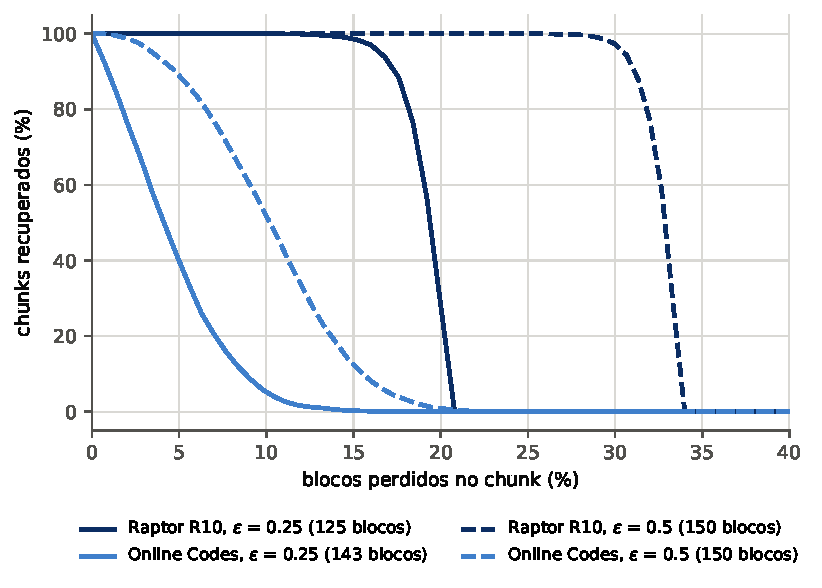
\includegraphics[width=\linewidth]{figuras/resultados/codec_loss.pdf}
	\end{columns}
\end{frame}

% ================================================================= Conclusão
\secao{Conclusão}{Ganhos, limitações e próximos passos}

\begin{frame}{Conclusão}
	\begin{columns}[T, onlytextwidth]
		\column{0.5\textwidth}
		\textbf{Ganhos}
		\begin{topicos}
			\item O R10 preserva MAC, Auditoria e Redistribuição.
			\item Mesmo custo, menos blocos, mais tolerância a perdas.
			\item Reparo limitado a um \emph{chunk}.
		\end{topicos}
		\column{0.46\textwidth}
		\textbf{Próximos passos}
		\begin{topicos}
			\item Evitar o cancelamento de erros no XOR.
			\item Ocultar a estrutura do código dos provedores.
			\item Códigos MDS e auditoria pública.
			\item Avaliação em nuvens reais.
		\end{topicos}
	\end{columns}
\end{frame}

\begin{frame}[standout]
	Obrigado!\\[1em]
	{\normalsize Perguntas?}
\end{frame}

% ================================================================= Apêndice
\appendix

\begin{frame}{Referências}
	\footnotesize
	\begin{itemize}\setlength{\itemsep}{0.5em}
		\item D. M. Amaral. \emph{Hy-SAIL: Uma nova abordagem para distribuição e armazenamento de informações em ambientes de computação em nuvem}. Tese de doutorado, UnB, 2013.
		\item D. M. Amaral et al. \emph{Hy-SAIL: Hyper-Scalability, Availability and Integrity Layer for Cloud Storage Systems}. IEEE Access, 2019.
		\item M. Luby. \emph{LT Codes}. FOCS, 2002.
		\item P. Maymounkov. \emph{Online Codes}. NYU, Relatório Técnico TR2002-833, 2002.
		\item A. Shokrollahi. \emph{Raptor Codes}. IEEE Trans. Inf. Theory, 2006.
		\item M. Luby et al. \emph{Raptor Forward Error Correction Scheme for Object Delivery}. RFC 5053, 2007.
		\item A. Juels, B. S. Kaliski. \emph{PORs: Proofs of Retrievability for Large Files}. ACM CCS, 2007.
		\item L. Clissa, M. Lassnig, L. Rinaldi. \emph{How big is Big Data?} Frontiers in Big Data, 2023.
	\end{itemize}
\end{frame}

\end{document}
